In the forthcoming deployment of WebRTC systems, we speculate that high
quality\footnote{normally, corresponds to increase in required bandwidth}
video confrencing will see wide adoption. Normally, to assure stability of the
network (and avoid congestion collapse), these real-time communication systems
will need to implement some kind of congestion control for their RTP-based
media traffic.

RTP transmits the media data over IP using a variety of transport layer
protocols such as UDP, TCP, and Datagram Congestion Control Protocol (DCCP).
Consequetly, congestion control for RTP-based media flows can be implemented
either in the application or the media flows are transmitted over congestion-%
controlled transport (TCP or DCCP). While using a congestion controlled
transport may be safe for the network, it is suboptimal for the media quality
unless the congestion-controlled transport is designed to carry media flows or
operates in a very low latency network ($<100$ms)~\cite{Brosh:tcp-real-time}.
On the other hand, using a non-congestion controlled transport (e.g., UDP),
the rate-adaptation is implemented in the application.  In this thesis, we
consider congestion control for unicast RTP traffic running over best-effort
IP network.

% CC should not cause queuing delay. Or define low-latency operation of
% multimedia cc.

Endpoints rely on RTCP feedback from the receiver to implement congestion
control. Hence, the congestion control should take into 3 aspects into its
design: congestion cues to report, block size of each report, and frequency of
these feedback reports. In the following subsections, we mainly discuss the
feedback reporting frequency, the classification congestion cues, requirements
of congestion control and lastly, criteria to evaluate congestion control
proposals.

\section{Congestion Cues}
\label{fw.cues}




\section{Congestion Reporting Frequency}
\label{fw.freq}

Normally congestion control requires a tight control loop, which means that
the receiving endpoint should be able to provide feedback at very short
intervals. Hence, the design of congestion control algorithm needs to be aware
of the limits on the timing of the feedback.  For example in TCP, the receiver
sends an \emph{acknowledgement} packet in response to every packet (or every
few packets) it receives. Whereas, RTCP encourages infrequent feedback and
specifies an upper-bound on the fraction of the session media bitrate that the
feedback packets can use\footnote{The specified feedback rate is $5\%$ for
each multimedia session}.  \cite{draft.rmcat.feedback} discusses three options
for the short report intervals, they are:

\textbf{Per-packet feedback report}: sends RTCP feedback every time the
endpoint receives a packet. For low bitrate media sessions (e.g., audio
streams) this would be quite difficult to achieve because the size of the
feedback packet would be comparable to the size of the media packet, i.e., the
feedback bitrate would larger than the $5\%$ fraction specified for it. If an
endpoint receives packets in a burts or at very short time intervals, the
endpoints will not be able to meet the timing requirements for per-packet
feedback because the RTCP timing interval calculation has a randomization
factor to avoid synchronizing feedback from multiple endpoints.

\textbf{Per-frame feedback report}: sends RTCP feedback every time the
endpoint recives a complete frame. This is mainly applicable to video where a
single video frame would be fragmented into multiple packets because the frame
size exceeds MTU size. Typically, an average size of an RTCP packet size in a
two-party call is $156$-$176$ bytes\footnote{The packet breakdown in bytes is:
UDP=16, IPv4=20 or IPv6=40, RTCP=8, SR=20, RR=24, SDES=28, one or more XR
blocks (20 each).}. For a 30 FPS biderectional video stream, the $rtcp\_bw
\approx 75$ \emph{kbps}, which requires the media session bitrate be set to a
value higher than $1.5$ \emph{Mbps} (to calculate assign the above values in
equation~\ref{eq:rtcp.int}). Consequently, it would not be possible to perform
per-frame for sessions with lower media rates. It should be noted that the
requirements for the media session butrate needs to be re-calculated if the
number of participants change, or the number of reported blocks change or the
frame rate changes.

\textbf{Per-RTT feedback report}: sends RTCP feedback at regular intervals
based on the RTT estimate. The requirement for the media session rate would be
lower, if the RTT is higher than the frame inter-arrival time. The calculation
of the RTCP interval for the per-frame still applies, except that the frame
rate is replaced by the RTT estimate.

To summarize, picking longer RTCP feedback intervals requires a lower media
session bitrate, which increases the area of operation (in terms of session
media rates).

\section{Classifying Congestion Cues}
\label{fw.fw}

A rate-control or congestion control algorithm relies on congestion cues to
pick a new sending rate. These cues can be observed at the receiver or by a
middlebox monitoring the flow, and it can also be aggregated by a
3$^{rd}$-party\footnote{A system outside the signaling or media path} or a
superpeer in an overlay network. Consequently, these observed cues need to be
signaled back to the sender which will perform congestion control. We classify
these congestion cues as a combination of \emph{where are they
measured/observed?}, and \emph{how is the sender notified?} For each there are
two options; In-path and Out-of-path \emph{sources} and In-band and Out-of-%
band \emph{signaling}. In-path congestion cues are measured by the receiver or
by middleboxes along the path. Out-of-path congestion cues are reported by
devices outside the media path (congestion maps, overlays, etc.). The
combination forms four cases, they are visualized in Figure~\ref{fig:4:fw}.

\begin{figure}[!h]
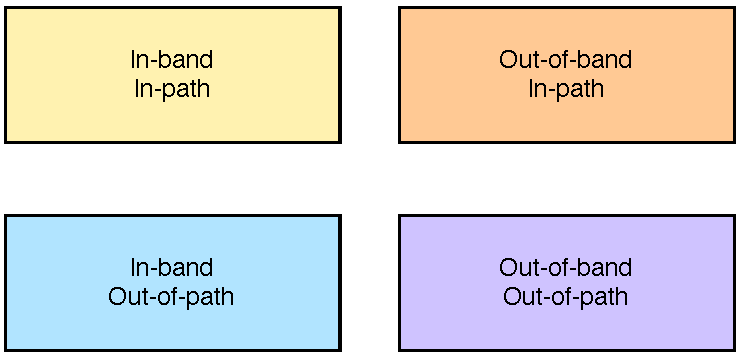
\includegraphics[scale=1.0]{chap2-fw-outline}
\caption{Classification of Congestion cues}
\label{fig:4:fw}
\end{figure}

A congestion control algorithm needs to pick one or more measurement points,
picking multiple adds to the feedback overhead and then choose a method to
signal it to the sending endpoint. It can choose to do it in-band by
encapsulating the cues either by piggybacking them on endpoint's own media
packets as RTP header extensions (this adds to the header overhead of a media
packet) or as RTCP extension blocks (see section~\ref{fw.freq} for details on
feedback frequency). Or the congestion control algorithm can choose to signal
the cues out-of-band, re-use the signaling path (e.g., SIP, XMPP) or setup an
alternate signaling path (e.g., HTTP or websockets). Following are the
examples for each category in the classification:

\textbf{a) In-path, In-band}: TFRC using information in RTCP RR, TMMBR.

\textbf{b) In-path, Out-of-band}: RTSP SPEED parameter, bandwidth parameter in
SDP, TFRC using additional loss reported by ECN markings.

\textbf{c) Out-of-path, In-band}: Multipath RTP (congestion on one path causes
change in per path fractional distribution.)

\textbf{d) Out-of-path, Out-of-band}: bandwidth information from congestion
maps, bandwidth lookup service, superpeers and overlays.

% monitoring: long-term, short-term

Another aspect to consider for classifying cues is the the measurement
duration to identify congestion, it can be over a long-term (order of seconds
or minutes) or a short-term (order of 100ms or a few seconds). For example,
jitter is measured on a per-packet basis, but reported over a longer
measurement interval (to filter for noise and transient delays).
Alternatively, packet losses, discards, etc. are measured over a shorter
interval so that the sender can react to these immediately.

\section{Congestion Control Evaluation}
\label{fw.cc.eval}

We need to define a set of requirements in order to design a congestion
control algorithm for multimedia. As a second step these requirements can be
used as a checklist to evaluate the suitability of the proposed algorithms.
Real-time interactive communication differs greatly from \emph{elastic}
traffic because the sender generates media packets in real-time and expects it
to be delivered in 100s of milliseconds and the receiver consumes the media
packets almost immediately, hence late arriving packets are useless.
Additionally, real-time communication systems can tolerate some amount of
packet loss and do not generate only constant bit rate streams but can adapt
the media rate over a fairly large range. \cite{draft.rmcat.req} lists a set
of requirements for RTP-based interactive multimedia sessions, these
requirements make up the guidelines described in~\cite{draft.rmcat.evaluate}.

In Section~\ref{rg.title}, we describe the scenarios in which to evaluate
congestion control, namely, when the flows are a) alone, b) competing with
self-similar flows, and c) competing with TCP flows (short-, long-lived) on a
bottleneck link.

These scenarios can be described as network topologies with varying link and
router characteristics, they are:

\textbf{Network topology}:

\textbf{Link characteristics}:

\textbf{Router characteristics}:


% Flow scenarios
% Link properties
% Router properties